\documentclass{beamer}
\usepackage[utf8]{inputenc}

\usetheme{Madrid}
\usecolortheme{default}
\usepackage{amsmath,amssymb,amsfonts,amsthm}
\usepackage{mathtools}
\usepackage{txfonts}
\usepackage{tkz-euclide}
\usepackage{listings}
\usepackage{adjustbox}
\usepackage{array}
\usepackage{tabularx}
\usepackage{gvv}
\usepackage{lmodern}
\usepackage{circuitikz}
\usepackage{tikz}
\usepackage{graphicx}

\setbeamertemplate{page number in head/foot}[totalframenumber]

\usepackage{tcolorbox}
\tcbuselibrary{minted,breakable,xparse,skins}



\definecolor{bg}{gray}{0.95}
\DeclareTCBListing{mintedbox}{O{}m!O{}}{%
  breakable=true,
  listing engine=minted,
  listing only,
  minted language=#2,
  minted style=default,
  minted options={%
    linenos,
    gobble=0,
    breaklines=true,
    breakafter=,,
    fontsize=\small,
    numbersep=8pt,
    #1},
  boxsep=0pt,
  left skip=0pt,
  right skip=0pt,
  left=25pt,
  right=0pt,
  top=3pt,
  bottom=3pt,
  arc=5pt,
  leftrule=0pt,
  rightrule=0pt,
  bottomrule=2pt,
  toprule=2pt,
  colback=bg,
  colframe=orange!70,
  enhanced,
  overlay={%
    \begin{tcbclipinterior}
    \fill[orange!20!white] (frame.south west) rectangle ([xshift=20pt]frame.north west);
    \end{tcbclipinterior}},
  #3,
}
\lstset{
    language=C,
    basicstyle=\ttfamily\small,
    keywordstyle=\color{blue},
    stringstyle=\color{orange},
    commentstyle=\color{green!60!black},
    numbers=left,
    numberstyle=\tiny\color{gray},
    breaklines=true,
    showstringspaces=false,
}
%------------------------------------------------------------
%This block of code defines the information to appear in the
%Title page
\title %optional
{2.4.21}
\date{August 24,2025}
%\subtitle{A short story}

\author % (optional)
{Harsha-EE25BTECH11026}



\begin{document}


\frame{\titlepage}
\begin{frame}{Question}
The number of vectors of unit length perpendicular to the vectors $a = 2\hat{i} + \hat{j} + 2\hat{k}$ and $b = \hat{j} + \hat{k} $ is
\end{frame}



\begin{frame}{Theoretical Solution}

Given the two vectors,
\begin{align}
    \vec{a}=\myvec{2\\1\\2} \;\;\; \vec{b}=\myvec{0\\1\\1}
\end{align}
we need to find the unit vector which is perpendicular to the vectors $\vec{a}$ and $\vec{b}$.The vector perpendicular to $\vec{a}$ and $\vec{b}$ is given by their cross-product.\\
\end{frame}

\begin{frame}{Theoretical Solution}
Let the perpendicular vector be $\vec{x}^T=\myvec{x_1&&x_2&&x_3}$
\begin{align}
    \because \vec{a}^T\vec{x}=0\\
    \vec{b}^T\vec{x}=0\;,
\end{align}
\begin{align}
    \therefore \myvec{\vec{a}^T\\\vec{b}^T}\vec{x}=0
\end{align}
\end{frame}

\begin{frame}{Theoretical Solution}
\begin{align}
    \myvec{2&&1&&2\\0&&1&&1}\myvec{x_1\\x_2\\x_3}=0
\end{align}
This can be represented as,
\begin{align}
    \myvec{2&&1&&2\\0&&1&&1}
    \xleftrightarrow{\,R_1 \gets R_1-R_2}
    \myvec{2&&0&&1\\0&&1&&1}
\end{align}
yielding,
\begin{align}
    2x_1+x_3=0\\
    x_2+x_3=0
\end{align}
\begin{align}
    \vec{x}=x_3\myvec{\frac{-1}{2}\\-1\\1}=\frac{x_3}{2}\myvec{-1\\-2\\2}
\end{align}
\end{frame}

\begin{frame}{Theoretical solution}
    As we know that the vector can be in both the directions i.e, into and out of the plane containing $\vec{a}$ and $\vec{b}$, so the vector perpendicular to vectors $\vec{a}$ and $\vec{b}$ would be $\pm\;(\vec{a} \times \vec{b})$.\\
\\
The desired output is
\begin{align}
    \vec{x}=\pm\frac{1}{3}\myvec{-1\\-2\\2}
\end{align}
\end{frame}

\begin{frame}[fragile]
    \frametitle{C Code - Cross product and magnitude of vector}

    \begin{lstlisting}
#include<stdio.h>
#include<math.h>

double find_magnitude(double *result)
{
	double mag;
	mag=sqrt(pow(result[0],2)+pow(result[1],2)+pow(result[2],2));
	return mag;

}
    \end{lstlisting}
\end{frame}

\begin{frame}[fragile]
  \frametitle{C Code - Cross product and magnitude of vector}
  \begin{lstlisting}
double find_cross_product(double *a, double *b, double *result)
{
    float A[2][3];
    float x1, x2, x3;
    // Build the 2x3 matrix [a; b]
    for(int j = 0; j < 3; j++) {
        A[0][j] = a[j];
        A[1][j] = b[j];
    }
    // Row reduction
    if (fabs(A[0][0]) < 1e-6) {
        for(int j = 0; j < 3; j++) {
            float tmp = A[0][j];
            A[0][j] = A[1][j];
            A[1][j] = tmp;
        }
    }


  \end{lstlisting}
    
\end{frame}
\begin{frame}[fragile]
    \frametitle{C Code - Cross product and magnitude of vector}

    \begin{lstlisting}

    float factor = A[1][0] / A[0][0];
    for(int j = 0; j < 3; j++) {
        A[1][j] -= factor * A[0][j];
    }

    // Solve system A * x = 0 with free variable x3 = 1
    x3 = 1;
    if (fabs(A[1][1]) > 1e-6) {
        x2 = -(A[1][2] * x3) / A[1][1];
    } else {
        x2 = 0;
    }
    x1 = -(A[0][1]*x2 + A[0][2]*x3) / A[0][0];

    result[0] = x1;
    result[1] = x2;
    result[2] = x3;

}
    \end{lstlisting}
\end{frame}

\begin{frame}[fragile]
    \frametitle{Python+C Code}
    \begin{lstlisting}
import numpy as np
import matplotlib as mp
mp.use("TkAgg")
import matplotlib.pyplot as plt
import ctypes

# Load shared library
lib = ctypes.CDLL("./libcrsproduct_mag.so")   # <-- change name if your .so file is different

# Define argument and return types for the C functions
lib.find_cross_product.argtypes = [
    ctypes.POINTER(ctypes.c_double), 
    ctypes.POINTER(ctypes.c_double), 
    ctypes.POINTER(ctypes.c_double)
]
lib.find_cross_product.restype = None   # because result is returned via array




    \end{lstlisting}
\end{frame}

\begin{frame}[fragile]
    \frametitle{Python+C Code}
    \begin{lstlisting}
lib.find_magnitude.argtypes = [ctypes.POINTER(ctypes.c_double)]
lib.find_magnitude.restype = ctypes.c_double

def cross_via_c(a, b):
    a_arr = (ctypes.c_double * 3)(*a)
    b_arr = (ctypes.c_double * 3)(*b)
    result = (ctypes.c_double * 3)()

    lib.find_cross_product(a_arr, b_arr, result)

    return np.array([result[0], result[1], result[2]], dtype=float)

a = np.array([2, 1, 2], dtype=np.int32)
b = np.array([0, 1, 1], dtype=np.int32)

    \end{lstlisting}
\end{frame}

\begin{frame}[fragile]
    \frametitle{Python+C Code}
    \begin{lstlisting}
# Cross product from C
x = cross_via_c(a, b)
print("Cross product :", x)

# Magnitude from C
x_ctypes = (ctypes.c_double * 3)(*x)
mag = lib.find_magnitude(x_ctypes)

# Unit vector
u = x / mag

print("Unit vector perpendicular to vectors a and b is \u00B1 [" + ", ".join(f"{val:.2f}" for val in u) + "]")
print("That is,")
print("+u =", [format(val, ".2f") for val in u])
print("-u =", [format(val, ".2f") for val in -u])

    \end{lstlisting}
\end{frame}

\begin{frame}[fragile]
    \frametitle{Python+C Code}
    \begin{lstlisting}
# --- Plotting ---
fig = plt.figure(figsize=(8,8))
ax = fig.add_subplot(111, projection='3d')

# Origin
origin = np.zeros(3)

# Plot a, b, and cross product directions
ax.quiver(*origin, *a, color='r', label='a', arrow_length_ratio=0.1)
ax.quiver(*origin, *b, color='g', label='b', arrow_length_ratio=0.1)
ax.quiver(*origin, *u, color='c', label='(a × b)', arrow_length_ratio=0.1) 
ax.quiver(*origin, *-u, color='b', label='-(a × b)', arrow_length_ratio=0.1)
    \end{lstlisting}
\end{frame}
\begin{frame}[fragile]
    \frametitle{Python+C Code}
    \begin{lstlisting}
ax.set_xlim([min(a[0], b[0], u[0], -u[0], 0),
             max(a[0], b[0], u[0], -u[0], 0)])

ax.set_ylim([min(a[1], b[1], u[1], -u[1], 0),
             max(a[1], b[1], u[1], -u[1], 0)])

ax.set_zlim([min(a[2], b[2], u[2], -u[2], 0),
             max(a[2], b[2], u[2], -u[2], 0)])

ax.set_xlabel('X')
ax.set_ylabel('Y')
ax.set_zlabel('Z')
ax.legend()
plt.savefig("/home/user/Matrix/Matgeo_assignments/2.4.21/figs/Figure_1.png")
plt.show()

    \end{lstlisting}
\end{frame}

\begin{frame}[fragile]
    \frametitle{Python Code}
    \begin{lstlisting}
import numpy as np
import matplotlib as mp
mp.use("TkAgg") 
import matplotlib.pyplot as plt

def cross_via_row_reduction(a, b):
     A = np.array([a, b], dtype=float)   # 2x3 system
    
    # Row reduction manually
    # Step 1: make pivot in first column
     if A[0,0] == 0:
         A[[0,1]] = A[[1,0]]   # swap rows if needed
    
    # Eliminate below
     factor = A[1,0] / A[0,0]
     A[1] = A[1] - factor*A[0]

    \end{lstlisting}
\end{frame}

\begin{frame}[fragile]
    \frametitle{Python Code}
    \begin{lstlisting}
 # Now we have 2 equations in 3 variables => free variable (say x3 = t)
    # Solve system Ax=0
    # Extract coefficients
     eq1 = A[0]
     eq2 = A[1]
    # Free variable x3 = t
     t = 1  # choose t=1 for direction
    # Solve eq2 for x2 in terms of t
     if abs(eq2[1]) > 1e-12:
        x2 = -(eq2[2]/eq2[1])*t
     else:
        x2 = 0
    # Solve eq1 for x1
     x1 = -(eq1[1]*x2 + eq1[2]*t) / eq1[0]
     return np.array([x1, x2, t])



    \end{lstlisting}
\end{frame}

\begin{frame}[fragile]
    \frametitle{Python Code}
    \begin{lstlisting}
# Given vectors
a = np.array([2, 1, 2], dtype=np.int32)
b = np.array([0, 1, 1], dtype=np.int32)

x = cross_via_row_reduction(a, b)
print("Cross product :", x)
mag = np.linalg.norm(x)

u=x/mag

print("Unit vector perpendicular to vectors a and b is \u00B1 [" + ", ".join(f"{val:.2f}" for val in u) + "]")
print("That is,")
print("+u =", [format(val, ".2f") for val in u])
print("-u =", [format(val, ".2f") for val in -u])

    \end{lstlisting}
\end{frame}

\begin{frame}[fragile]
    \frametitle{Python Code}
    \begin{lstlisting}
# --- Plotting ---
fig = plt.figure(figsize=(8,8))
ax = fig.add_subplot(111, projection='3d')

# Origin
origin = np.zeros(3)

# Plot a, b, and cross product
ax.quiver(*origin, *a, color='r', label='a', arrow_length_ratio=0.1)
ax.quiver(*origin, *b, color='g', label='b', arrow_length_ratio=0.1)
ax.quiver(*origin, *-u, color='b', label='-(a × b)', arrow_length_ratio=0.1)
ax.quiver(*origin, *u, color='c', label='(a × b)' , arrow_length_ratio=0.1) 
    \end{lstlisting}
\end{frame}

\begin{frame}[fragile]
    \frametitle{Python Code}
    \begin{lstlisting}
ax.set_xlim([min(a[0], b[0], u[0], -u[0], 0),
             max(a[0], b[0], u[0], -u[0], 0)])

ax.set_ylim([min(a[1], b[1], u[1], -u[1], 0),
             max(a[1], b[1], u[1], -u[1], 0)])

ax.set_zlim([min(a[2], b[2], u[2], -u[2], 0),
             max(a[2], b[2], u[2], -u[2], 0)])


ax.set_xlabel('X')
ax.set_ylabel('Y')
ax.set_zlabel('Z')
ax.legend()
plt.savefig("/home/user/Matrix/Matgeo_assignments/2.4.21/figs/Figure_1.png")
plt.show()

    \end{lstlisting}
\end{frame}

\begin{frame}{Plot}
    \centering
    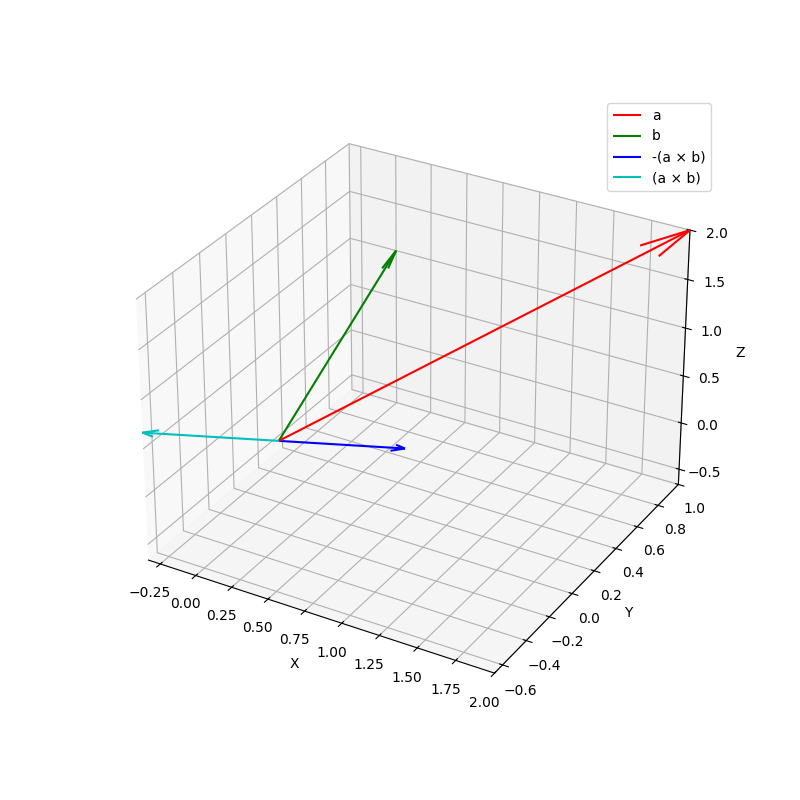
\includegraphics[width=\columnwidth, height=0.8\textheight, keepaspectratio]{figs/Figure_1.png}     
\end{frame}




\end{document}